\documentclass{article}
\usepackage[utf8]{inputenc}

\title{2D Segment Trees}
\author{Joshua Zhang}
\date{March 2020}

\usepackage{graphicx}
\graphicspath{ {./images/} }
\begin{document}

\maketitle

\section{Introduction}
    \hspace*{1em} \quad Most of us are familiar with range queries in a 1D context. However, there are times where we may need to run these same queries in a 2D scenario. Let's look at ways we can modify the algorithms that we know: prefix sums and segment trees, to work in two dimensions.
    
\section{2D Prefix Sums}
    \subsection{Introduction}
    \hspace{1em} \quad Before we jump into 2D segment trees, let's look at a much simpler algorithm. In the case where we don't need to update points, 2D prefix sums will suffice.
    
    \subsection{Explanation}
    \begin{figure}[h]
        \centering
        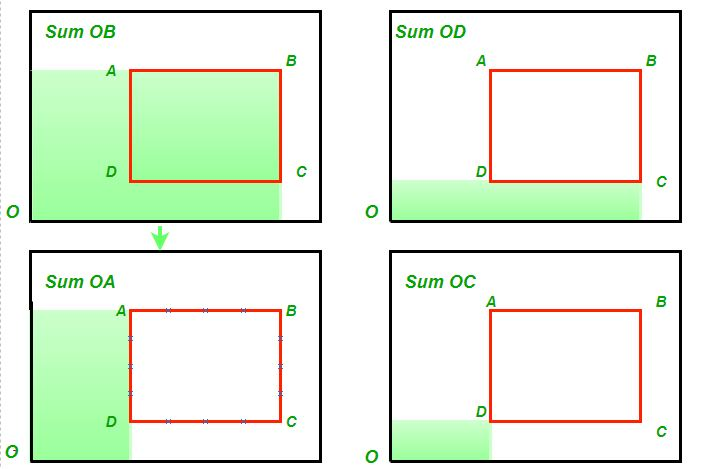
\includegraphics[scale = 0.45]{Images/image1.jpeg}
        \caption{The 4 sums we need to make for each query, (Credit: GeeksForGeeks)}
    \end{figure}
    
    \hspace{1em} \quad Similar to prefix sums, we will keep an array $A$ where $A[i][j]$ represents the sum of all elements between $i, j$ and the corner of the rectangle. In order to calculate this efficiently, we'll use the equation $A[i][j] = A[i-1][j] + A[i][j-1] - A[i-1][j-1]$. Note that we subtract $A[i-1][j-1]$ to prevent double counting. In order to query, we'll take the prefix sums outlined in Figure 1. The sum of rectangle $abcd$ is $A[i_b][j_b] - A[i_a][j_a] - A[i_c][j_c] - A[i_d][j_d]$.
    
    \subsection{Complexity}
    N and M are the lengths of the sides of the rectangle
    \begin{itemize}
      \item Creating the Prefix Sums: $O(NM)$
      \item Querying for a rectangle: $O(1)$
      \item Updating the Prefix Sums: $O(NM)$
    \end{itemize}
    
\section{2D Segment Trees}
    \subsection{Introduction}
    \hspace{1em} \quad While prefix sums work for a lot of 2D range queries, there are times where we will have to update our values. In order to support this, we'll utilize a 2D segment tree.
    
    \subsection{Explanation}
    \hspace{1em} \quad Most of us are familiar with the 1 dimensional segment tree. Usually, a segment tree will be a binary tree of values. For a 2D segment tree, we'll make a tree of trees instead. Each node in our tree will no longer be a value, but rather a entire segment tree. If we imagine our values as a rectangle, each leaf of our tree will correspond to a row and Parent nodes will correspond to sub rectangles. When we query, we will find the segment trees corresponding to the rows that we want, and then query for the column values from those segment trees. For range updates, just do lazy propagation instead of querying. Instead of updating the values at each node directly like in a normal segment tree, however, we will run a range update on the segment tree at each node.
    
    \begin{figure}[h]
        \centering
        \includegraphics[scale = 0.4]{Images/image2.png}
        \caption{A grid of values, (Credit: GeeksForGeeks)}
    \end{figure}
    
    \begin{figure}[h]
        \centering
        \includegraphics[scale = 0.35]{Images/image3.png}
        \caption{The segment tree corresponding to Figure 2, (Credit: GeeksForGeeks)}
    \end{figure}
    
    \hspace{1em} \quad As we can see in the figures above, each leaf of the 2D segment tree is a segment tree of the rows of the grid. The parents nodes are segment trees of the sum of the values of it's children. 
    
    \subsection{Complexity}
    N and M are the lengths of the sides of the rectangle
    \begin{itemize}
      \item Creating the Segment Tree: $O(NM)$, each node segment tree takes $O(M)$ time to build, and there will be $O(N)$ nodes total in our tree
      \item Querying for a rectangle: $O(\log N \log M)$, $O(\log N)$ to find the nodes corresponding to the first dimension, $O(\log M)$ to query from each of those nodes.
      \item Updating the segment tree: $O(\log N \log M)$, $O(\log N)$ for update in the first layer, $O(\log M)$ for updates in the second.
    \end{itemize}
    
\section{Example Problem}
    USACO 2016 January Contest, Platinum - Problem 2. Mowing the Field

\end{document}
